\pdfoutput=1

\documentclass{l4proj}
\usepackage{graphicx}
\graphicspath{{images/}}
%
% put any packages here
%
\usepackage{natbib}
\begin{document}
\title{Social Networking with Project Task Management}
\author{Euan Parker}
\date{2015/2016}
\maketitle

\begin{abstract}

\end{abstract}

\educationalconsent
%
%NOTE: if you include the educationalconsent (above) and your project is graded an A then
%      it may be entered in the CS Hall of Fame
%
\tableofcontents
%==============================================================================

\chapter{Introduction}
\pagenumbering{arabic}


Project task management is typically done using a combination of ticketing systems, to formally record aspects about the project, and informal communication such as social networking, messaging tools or simply face to face discussion. This represents a duplication of effort whereby developers with discuss a task using an informal medium and then go on to record what has been done using the ticketing system.  As a result developers often become less diligent in using their management tools due to the perceived waste of time in recording information that has already been discussed elsewhere. 

Tearooms seeks to solve this problem by providing a platform which integrates a social networking platform with a ticketing system. This project was originally undertaken as a third year group project, but was continued as an individual fourth year project.  In this tool a conversation system is provided whereby meta-data can attached to each conversation in order to store additional information that relates to the topic.  Moreover a variety of metrics can be viewed regarding the chats, such as what chats are most active, what participants contribute the most or what chats has the most information per message.

There are a number of existing systems which adhere to the 'ticket-based management', 'conversation based management' and 'task management' paradigms, such as Jira, Slack, Trello and Trac.  These systems offer different approaches to management but none manage to properly integrate all the various approaches into one system.

The second chapter of this paper will discuss the research that was undertaken prior to beginning the project. In this a number of papers relating to the subject of software team management were studied.  These discussed the potential problems that can arise in these areas, such as the loss of information due to developers discussing their work informally and not documenting these talks, the difficulties in assigning tasks to the appropriate people and issues with globally distributed development teams.

In the third chapter it will be discussed the difficulties that arose in working with what was effectively a legacy system as a result of work that was undertaken over the summer.  During this time the entire front-end framework was re-written, meaning returning to the project in fourth year was a great challenge, as the system was in many ways completely different and thus past experience in developing the project was of limited use.  

The fourth chapter will detail the work that was undertaken in the recent academic year and how that work contributes towards the aim of improving project task management. Specifically this will discuss what features have been added, and how these will assist with one of the issues identified in the previous chapter.

The fifth chapter will discuss the next logical steps for the project, and what work could be done in the future to fully realise the key aspects of the concept.


\chapter{Related Work}
A number of works were studied that related to the issue of team communication and team management.  These works covered a variety of topics pertaining to the field of management, namely that of 'Distributed Software Management', 'Task delegation', 'Informal versus formal communication' and 'Collaborative Techniques'.
%----------------------------------------------------------------------------

\section {Informal versus Formal Communication}

In a project environment people will tend towards using informal means of communication such as in person discussion, social media and phone calls.  It is discussed how this will mean there is a lot of information relating to the project that is produced by team members that is never formally recorded and thus is lost in time.  It is discussed the reasons for this reticence to record what is discussed, as well as potential solutions in order to better utilise the untapped resource of conversations.

It is discussed how the architecture of a system being developed often dictates how the team organisation will be split up.  It is proposed that this alone is not sufficient to fully coordinate a large development team, and taking into account different tasks, milestones, plans and processes must be considered to effectively manage a team.  It is said however that this is rarely successfully achieved in the real world, due to unpredictable factors in the development process such as inaccurate estimates, changing requirements, incomplete solutions and personnel leaving or joining the project.  

These problems are circumvented largely due to informal communication and organisation, whereby the developers will discuss components of their work while at lunch, on a break or over social media.

A case study was carried by \citet{herbsleb99architectures} on a technology department of a multinational country, which was chosen for the factor that sites in different countries had the added organisational complication of multiple languages.  The department was currently working on a project whereby different teams worked on different components of a large system, and simulated the rest of the system for the purpose of development.  It was found however that in creating the simulated components the problem description lacked certain essential details and as a result each team had made their own assumptions regarding missing information.  As a result each team ended up with different assumptions and when the components were integrated they did not work correctly.  It was found that team members were reluctant to record these assumptions as they viewed it as taking away from time that could be spent developing the system, when they had already discussed it within their teams.

It is discussed how Concurrent Version Systems (CVS) can be used in the organisation of software development. These can serve to manage the software itself, and additional information can be attached to commits to record information.  However, \citet{fitzpatrick06cvs} proposes that these do not encapsulate the informal discussions regarding the code and thus could stand to be augmented by the addition of a lightweight event notification system.  This tool would display messages from the CVS and offer a chat system for developers to discuss them, thus allowing for a combination of formal documentation and informal discussion.

In a paper by \citet{malone94interdisciplinary} a survey on coordination theory is documented, which details the problem of communication in a development group.  The motivating question of this is "How will the widespread use of information technology change the ways people work together?"

This is a relevant question due the the in computers that are used for coordinating work, and how the improvements in information technologies are allowing for greater communication and coordination.

It is stated that in order to best aid coordination, work should be done in order to improve
\begin{enumerate}
\item designing tools to enable people to work together
\item properly utilise multiple computers processing power to work on related problems
\item creating more flexible ways of organising collective activity.
\end{enumerate}

A system was produced by \citet{handel02chat} on a synchronous messaging application with support for group discussions.  This tool was used by teams in a workplace to discuss a project currently being worked on via text. It was found that despite text persisting for one day, the tool was mostly used in bursts of synchronous discussion with only occasional asynchronous exchanges, meaning discussions were mostly conducted in real time with immediate responses, instead of leaving a message as a note to be responded to when appropriate. 

\citet{cubranic03hipikat} discusses how as a result of distributed development teams new members of such companies cannot learn from their experiences colleagues, due to absence of informal encounters. The paper proposes a solution through a tool that provides a "project memory".  The tool helps newcomers working on a task find similar examples in the source code from previous work done. 

To solve this problem a tool was developed, named a 'workspace awareness tool' which provides developers insight into other workspaces.  Specifically it informs developers when other developers change related artefacts.  These notifications show the severity and effect of changes, and allow developers to work around what has been changed in advance.

It is discussed that projects with a globally distributed development team informal communication is severely limited, resulting in difficulty in spreading tactic knowledge.  This knowledge is what allows for a full overview of an organisation and thus all participants do not have access to the rational behind decisions.  As a result when problems arise it can take days to rectify despite the issues being easily rectifiable if the relevant stakeholders were identified.

\citet{bruegge06sysiphus} proposes a system that captures information about organisational roles and structures it for use.  The system encourages participants to make communication and issues explicit in the system models and thus relevant stakeholders are identified.  This means when people are working on a part of the system Sysiphus can display what other users have worked on that particular section.

With the increase in scale and distribution of software development the shared understanding that developers would historically built up is more difficult to attain, as this originally would have come about through formal and informal face-to-face meetings and gatherings.  Thus \citet{omoronyia09developer} proposes a model that seeks to encapsulate the ordering of tasks, artefacts and developers relevant to particular work contexts in projects.  This model would be built up using data gathered from the developers interactions with IDEs.  Specifically it would identify entities (developers, tasks, artefacts), associated with a particular work context, then identify relationships among these. Furthermore some information can be acquired regarding where developers work, and when.

%----------------------------------------------------------------------------

\section {Distributed Software Development}

It is discussed as to how best manage a geographically distributed software development team, meaning a team which may have multiple members or sub-teams separated by a great distance, or perhaps even in different countries.  This links back to the previous section, as due to this separation it is usually impossible to have face to face meetings with other team members, and informal interaction is severely limited.   As a result the amount of working information that is usually generated about a project, through team members getting to know each others strengths and weaknesses, will not build up.  Moreover, there arise difficulties in communication, as without frequent discussion the different teams may differ in their objectives or interpretations as to what has to be done.  This can also occur due to language or cultural differences.


There is a rising trend of software development projects to have multiple teams in different locations, often even different continents.  This is due to the increased ease of communication over long distances as well as the accessibility of skilled workers regardless of where they live.

\citet{herbsleb07global} finds however that many of the usual aspects of co-located projects are lost in a distributed team, whereby through frequent, informal interactions team members get to know the skills and expertise of their team members.  Ideas are also more effectively communicated when teams share a common native language as there is less chance of misunderstandings, or ideas that are difficult to communicate.

As a result globalisation is considered by some to be one of the major research challenges in requirements engineering.  Suggested solutions were improving communications and more disciplined project management such as assigning roles and frequently documenting what has been done

Software development tools are primarily focused on assisting the technical side of development, despite the fact that large parts of the process are organisational tasks.

\citet{halverson06designing} discusses that software development was originally conducted in such a way whereby all code would be developed in one place, then over time it would be maintained by other people in different locations, thus communication between developers could be done via comments in the code.  Now however this has evolved such that it is now commonplace to have distributed development teams and a variety of communication methods to support the development and maintenance of systems.  With small local teams physically walking into someone's office is often the best way to discuss something, but this is not possible for larger scale companies.

Another issue identified is the visualisation of the development of software.  It is proposed that visualising data gathered from version control could be used to identify trends in the evolution of very large software systems, for example to identify candidates for re-factoring.  

a case study made was one whereby participants of a project were represented by a coloured hexagon.  The colour represented the status of the person in relation to a task (e.g. in progress, completed or not started)
The hexagons were arranged according to their position within the organisation.  This allowed for an overview of the participants to be easily viewed as well as what tasks were completed.

There are a number of necessary differences in organising a virtual team (i.e. geographically distributed) versus organising a collocated team.  Geographic, temporal, cultural and linguistic distance all hinder coordination, cooperation and communication. 

\citet{casey10virtual} states that global projects carry additional risk of delay or failure due to linguistic and cultural difference, motivational differences and temporal distance.  The paper proposes how best to organise a virtual team in order to prevent this.  It is essential to formalise roles, relationships and rules to aid in communication and control.  This process must be documented and formalised in order to ensure these are followed. 

In distributed development teams it is inevitable that as a result of so many different developers in so many different places a huge knowledge base will be created but is largely inaccessible.  \citet{bass07collaborative} proposes a system to gather this information and compiling it in a form that is more accessible.

This information was gathered through semi-structured interviews whereby participants filled in a form describing a practice they employed in dealing with a Global Software Development related issue that had been successful.  It was proposed that a good way to share the information could be

\begin{itemize}
\item \textit{Distributed Pair Programming} \par
Two geographically separated members of the team practice virtual pair programming together, jointly reviewing software and making changes where necessary.  Through this link a reciprocal relationship is established whereby information and knowledge will be shared.
\item\textit{Urgent Request} \par
A broadcast mechanism for requesting information pertaining to a project.  This relies upon project members volunteering themselves as a contact for specific topics, and aims at promoting unplanned communication in the case that there arises an urgent need for information about a particular aspect of the project.
\end{itemize}


Distributed development can actually increase the time it takes for the development of individual tasks, such as requests for modifications.  This can be attributed to the amount of people involved and the time taken to contact these people (who may even be in different time zones) can add large amounts of time to tasks.  

In order to solve this \citet{herbsleb03empirical} proposes that tasks must be decoupled from each other and distributed based on location, such that different development sites can work independently of each other.

Alternatively increased use of communication technology allows for an approximation of same-site communication through thorough documentation of what has been done.

There are a number of proposed practices that aid global development projects.  \citet{paasivaara03collaboration} carried out a case study was carried out over the scope of 8 different globally operating projects.  34 Semi-structured interviews were carried out and from these it was gleaned that collaboration practices such as milestone synchronisation, frequent deliveries and establishing peer-to-peer links are often identified (by interviewees) to be successful. 

It was also found that planning for problem-solving communication was often neglected early on in a project.  In order to fix this the use of bulletin boards or e-mail lists is suggested.  This could also apply to a software-based fix whereby a ticket is created for all related problems to be posted to.

\section {Task Delegation}

In most systems it is necessary to manually assign a user to resolve a task.  This can take up time unnecessarily as often research will have to be done into who is best suited to such a a task if it is not immediately obvious, and having to access the management software and assign them takes up time which could be spent on more important tasks.

%----------------------------------------------------------------------------
 
\citet{anvik06who} suggests a semi-automated way of assigning bug reports to a developer, through use of a machine learning algorithm.  This algorithm looks at an open bug repository in order to learn the kind of reports each different developer on the team resolves.  When a new bug report arrives the the system will then recommend a group of developers that could be expected to resolve this based on what they have done previously.
%----------------------------------------------------------------------------
\section {Collaborative Techniques}

This section details ways the software development process can be improved through use of better project management software.  This includes the suggestion of add-ons to existing systems, as well as tools that directly aid software development. Although the latter does not directly relate to project task management, concepts from these could be taken and integrated into task management tools.

\citet{whitehead07collaboration} discusses how collaboration techniques have evolved to remedy the limitations of memory. It is discussed how the goals of collaboration techniques are:

\begin {enumerate}
\item Establish scope of a project
\item Push the project towards an end result
\item Manage dependencies between artefacts in the project
\item Reduce dependencies among developers
\item Identify and solve errors
\item Record the time-line of the project
\end {enumerate}

In order to achieve these goals a number of technologies are adopted by software engineers.  These different technologies are used at different points in the development cycle, such as a single tool for the requirements phase, then another tool for creating UML diagrams, and so on.  It is proposed that the a future development could be a tool that can be used to cover all points in a software development cycle.

Moreover, \citet{storey09software} proposes an improvement to the concept of comments, whereby developers often add these annotations to source code to remind them of relevant information and mark locations of interest.  A tool was developed that supports semantically rich tagging whereby annotations to code are managed by the tool and can be browsed independently.  These annotations can be edited and created, as well as associated with pertinent pieces of code.  

This could also be taken the opposite way, whereby a ticketing system could integrate with a source code repository and support direct linking to parts of the code.


\citet{froehlich04unifying} proposed a tool that combines the two sources of complexity in software development - Code complexity and the complexity that comes with producing it.  This tool would provide a development environment in which both the code would be visible as well as activity that has recently been performed in relation to the code.

From looking at activity information in Github a large amount of information can be inferred pertaining to the persons technical aims and vision regarding a piece of code.  Moreover it can be used to guess a projects prospective success based on how regularly it is updated, and how supported a project is based on attention from the community.

\citet{dabbish12social} gathered information on this through semi-structured interviews on GitHub users, in order to document and understand how different aspects of GitHub's functionality were used.  The users were asked to walk through a session on GitHub and describe how they interpreted information displayed on the site.

%----------------------------------------------------

\section{Conclusion}

Based on previous research, there exist a number of issues with modern software management.  These issues stem from a variety of causes, such as the modes of communication between teams.  In this a large amount of information is lost due to the informal conversations between team members not being recorded.  This issue is further exemplified by the issues in distributed development.  In this situation a physical separation prevents the fostering of a familiarity with the other members of the development team.  This means it is more difficult to know other peoples strengths and weaknesses, as well as who to ask about specific topics. These such problems could stand to benefit from a system such as tearooms which seeks to integrate casual conversation with a ticketing system, thus using the information taken from the conversation and storing it as data.  Supporting management through casual conversation also assists in encouraging a working relationship between different team members in different places, meanwhile also ensuring proper documentation is taking place.

\chapter{Analysis of the existing system}

\section{Prior Work}

The project originally began as a third year group project.  The premise of the system was to create a tool that integrated social networking with project task management.  This was to provide an alternative approach to the traditional ticket management system so as to allow developers to focus on communication rather than spending time recording data in the system.  This primary focus of the system was identified due to the duplication of effort that currently exists in other systems.  This is defined as the repetition that occurs when a team discusses an issue on a different messaging platform, or in person, and then goes on to formally record this in a ticket.

The system had to closely integrate with a social networking feature in order to capture and process information gleaned from the users communication.  It was originally considered that the system would be a Skype extension, but the decision was made to create a chat system from scratch. 

The resultant system was built on the Django framework, which is a python web development framework.  The server side of the application was written in python, while the client side was written primarily with the 'Jquery' JavaScript library, and a number of other libraries to handle components such as the chat and graphs. 

\subsection{metadata}
The ability to attach metadata to conversations separates the software from normal messaging systems, and makes it suitable for project management.  It provides information to developers relating to the conversations and can be seen in the 'details' tab.  The metadata consisted of:

\begin{itemize}
\item \textit{Assignee} 
\par By default this is the user that created the conversation.  This can be changed manually from a dropdown list of all the other users
\item \textit{Cost}
\par This is an arbitrary number between 1 and 10 used to represent the effort needed to complete a task. 
\item \textit{due Date}
\par This refers to the date and time by which the conversation should be resolved
\item \textit{Notes}
\par This is a text field used to attach additional information to the ticket, such as linking to resources or websites. 
\item \textit{Saved Messages}
\par These are messages that have been sent in the conversation that, if marked as important, are saved to the details page. 
\item \textit{Priority}
\par This is a value used to denote the importance of of a conversation.  This field can be one of three values: 'High', 'Medium' or 'Low'.
\item \textit{Tags} 
\par Users can set tags to signify what topics are discussed within the conversation.  These are stored in the details tab as well as attached to the conversations entry on the project page.
\end{itemize}

\subsection{Statistics}

The visual representation of statistics related to the projects was a feature that was identified and started in the original project.  These provide an insight into the state of a project, allowing users to view the amount of activity within a project and the individual contribution of each participant.  These graphs were implemented using the d3 Javascript library.
In the original version of the system there were three graphs added:

\begin{itemize}
\item Messages sent per user in a conversation
\item Messages sent per user in a project
\item Messages contained in each conversation in a project
\end{itemize}

\subsection{Notifications}

The system provided notifications whereby users receive a message informing them that a chat they are participating in has new messages.  This was done as when a user is active in many chats it becomes very difficult, not to mention time consuming, to keep track of what is being discussed in each.  Each notification consists of a pop-up which shows the name of the chat that the message is in, as well as a preview of the message.

\subsection{Filtering and Sorting}

In large scale projects it can be difficult to find specific conversations.  To remedy this the ability to sort the conversations by priority and due date was implemented in order to better find particular conversations. 

Moreover users can filter the conversations, whereby the user enters a keyword and any conversation that does not have this in the title is hidden.  Similarly this was implemented in the conversations themselves, whereby messages can be filtered by a keyword, or by user.

\section{Working with a Legacy System}

Over the summer a subset of the original development team worked to completely re-write the front-end of the software.  The front-end was originally written using the JavaScript library 'JQuery'.  However, this was redone using the 'React' library.  Moreover, the original graphing library d3 was removed and the existing graphs were re-created in 'react-chartjs'.

This was done due as the speed limitations of JQuery were becoming an issue on the already fairly cumbersome system.  React was found to be much faster, and as a more modern technology seemed a useful tool to be acquainted with.  Moreover, react seemed to be well suited to the project, as the component based architecture integrated well with the project's module-based interface whereby different elements on the screen are each contained in different sections.

As a result of these changes, when beginning the project implementation was delayed as a result of having to learn the changes in the system.  This time was spent reading through the code itself, as well as getting in contact with the previous developers in order to question them about how certain components worked.  Moreover, over the course of the project there were recurring problems working with legacy code.  This often arose from difficulties in comprehending what a certain part of code did, sometimes as a result of poor or incomplete documentation.

\chapter{Features}

The 'tearooms' project was started with the aim of tackling a number of identified issues with current task management systems. A common problem with systems such as this is that users have to spend a lot of time recording information.  This is time that could otherwise be spent developing, or doing other important tasks.  In order to help alleviate this a number of tools are provided, such as being able to change meta-data attributes through the chat, or saving messages to the details tab for future reference.   Another issue is that of knowing who should do what.  In response it is proposed that this sort of information can be found through data analytics, as looking at metrics such as users previous work and who they work with can paint a picture of the sort of developer they are.  This information can be used to suggest users to add to a conversation, or to recommend to a user what sort of project they might be interested in.

Previously the workflow when using project management software would resemble something like figure \ref{fig:1}.  


\begin{figure}[h]
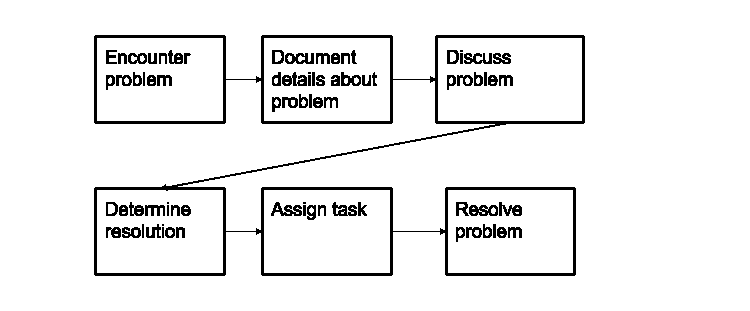
\includegraphics[scale=0.75]{old-workflow.png}
\centering
\caption{Normal workflow for project task management}
\label{fig:1}
\end{figure}
\newpage

However, tearooms looks to simplify the process by eliminating as many unnecessary steps as possible, or automating a step if possible. The ability to save information to metadata as a topic is discussed, and the system generating automated recommendations works to remove the need for documenting issues, or assigning tasks.  As a result an ideal workflow could look more like figure \ref{fig:2}. 

\begin{figure}[h]
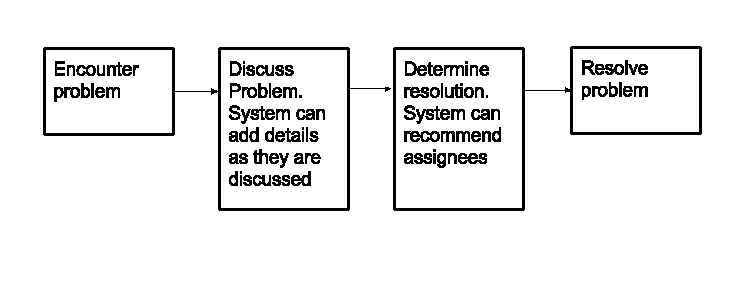
\includegraphics[scale=0.75]{New-workflow.png}
\centering
\caption{Tearooms proposed workflow for project task management}
\label{fig:2}
\end{figure}

\section{Graphs}

It was found that graphs could be used to monitor the progress of a project. The data in the graph can often reflect the state of the project or conversation it pertains to when compared to other similar examples.

\begin{itemize}
\item \textit{A graph of messages over time per chat}
\par This can show which chats are currently being actively worked on, as well as showing which have been worked on - and to what extent - over the last week.  This information can be used to determine how well a task is going, or if it is nearing completion.
\item \textit{A graph of content over time per chat (\ref{fig:3})}
\par This can be compared with the graph of messages over time to determine which chats have longer messages.  In situations where two chats have similar amounts of messages but one has significantly more 'content' it could be true that a more detailed discussion is taking place in this chat.
\item \textit{Number of messages over time per participant}
\par This can be used to determine an individuals contributions over time.  For example, a user with low contributions recently may be struggling with their current work, or have been busy lately. Alternatively a user with low contributions overall may not be working as hard, or may be less diligent in using project management software.

\end{itemize}



\newpage


A number of graphs with sample data were added.  A working example was not able to be completed in the timespan of the project and thus these were created in order to demonstrate the information that could be gleaned from these examples.  These example graphs are as follows:

\begin{itemize}
\item \textit{Number of messages per day per participant}
\par This can be used to view what users participate more in discussions, as well as being able to view trends in discussions such as on what days users are most active.
\item \textit{Content per day per participant (\ref{fig:4})}
\par This can be used in conjunction with the previous graph to ascertain the quality of messages.  For example, a high amount of messages with low total characters implies a lot of short answers, while a few messages but lots of characters may mean a detailed post.\item \textit{Number of message type per day}
\par This denotes what type of conversation the message is posted in, e.g. the majority of comments could be in conversations tagged with "bug".  This can be used to gain an overview of a project by showing what type of conversations go on.  For example, if the majority of discussions are about documentation the project may be nearing the end of development, whereas if many are discussing features then there is a good chance it is in the middle of the implementation phase.
\end{itemize}

\begin{figure}[h]
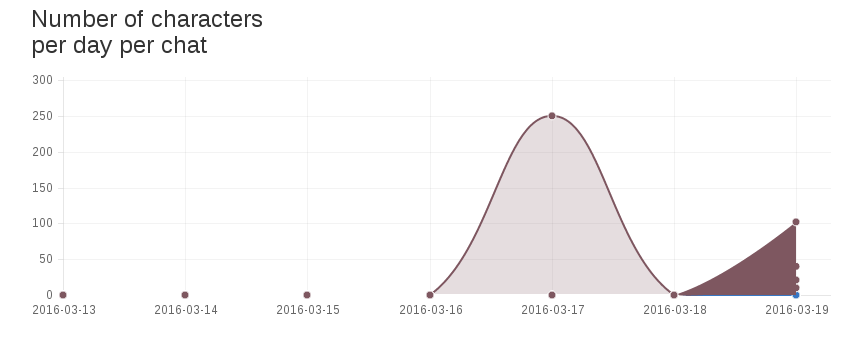
\includegraphics[scale=0.75]{WorkingGraph.png}
\centering
\caption{Graph of content over time per chat}
\label{fig:3}
\end{figure}


\begin{figure}[h]
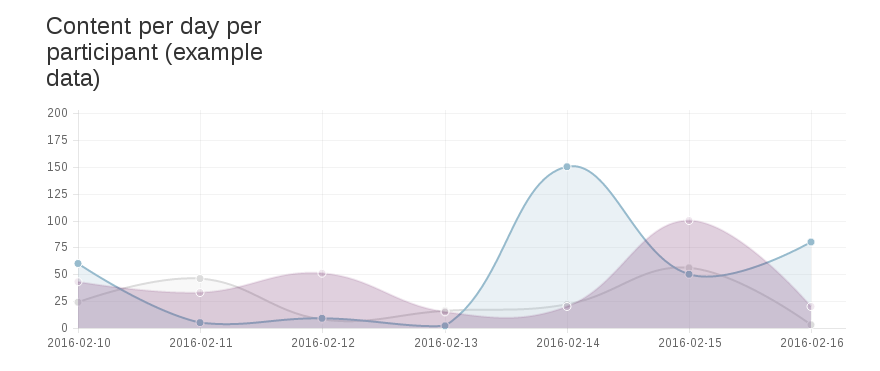
\includegraphics[scale=0.75]{SampleGraph.png}
\centering
\caption{Example graph of content over time per participant}
\label{fig:4}

\end{figure}

\newpage
Sample graphs were also created for the user profile page, whereby the information would reflect upon the user and provide an insight into what sort of topics they frequently discuss. These graphs where:

\begin{itemize}
\item \textit{Contributions per project over time} 
\par This shows which projects the user participates in, and how much they contribute over the last week.  This can be used to determine which projects are currently worked on the most by the user.
\item \textit{Total Contributions}
\par This shows the total amount of messages the user has posted in all the projects, and can show which projects they have been most involved in.
\item \textit{Who do I talk to}
\par This can be used to identify other users the current user frequently talks to.  This may be of interest as if someone has taken an interest in what the user frequently works on this can direct them to other people who work on similar projects.
\item \textit{Types of conversations involved in}
\par This shows what sort of topic the user most frequently posts in, and thus reveals what areas they are likely to be most experienced in. 
\end{itemize}

\section{Editing Metadata through the Chat System}

Having to stop using the chat system in order to attach additional metadata is an inconvenience and one that breaks the natural flow of discussion.  In order to remedy this a number of chat commands were added to allow for users to alter the various metadata attributes by using certain symbols. When a certain symbol is used it is marked that the word that immediately follows is a phrase that represents a value to be stored in metadata, as seen in (\ref{fig:10})

\begin{figure}[h]
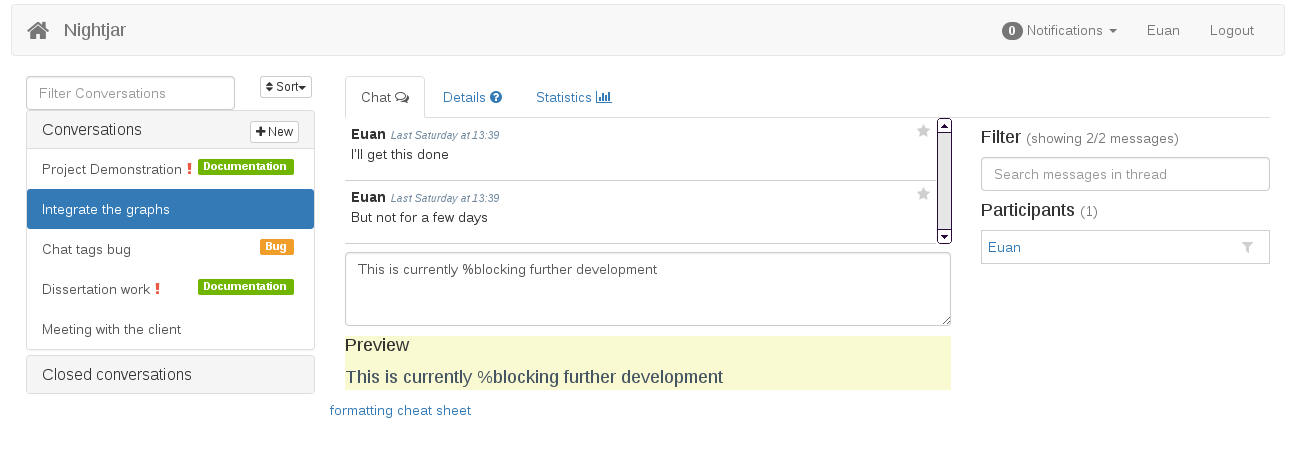
\includegraphics[scale=0.75]{chat-parsing.png}
\centering
\caption{Example of using chat parsing system}
\label{fig:10}
\end{figure}
\newpage

This example will set 'blocking' as one of the tags for the conversation.  This is done to further reinforce the idea of integration between a chat and ticketing system, allowing for users to change metadata in the middle of the conversation in a natural way, meaning they do not have to navigate to a separate page.  A formatting cheat sheet for the various commands was also added to help new users learn how to use the system.  A full list of chat commands are as follows:

\begin{itemize}
\item @username tags a user in a conversation.  The user will receive a notification informing them they have been tagged.
\item \%tag adds a tag to the conversation.  The possible tags are bug, feature, documentation, blocking and enhancement.
\item \$cost adds a cost to the conversation.  The cost is a number between 1 and 10.
\item \textasciicircum priority sets the priority of the conversation, which is either low, medium or high.
\end{itemize}

\newpage

\section{Data Analytics}
Additionally, a set of example features were added to demonstrate the potential use of data analytics for the system.  This included:

\begin{itemize}
\item \textit{Suggestions for related projects (\ref{fig:5})}
\par These could be generated by looking at aspects such as what is discussed in the conversations, who takes part in the conversations and what time these conversations were started
\item \textit{Suggested users to invite to the project}
\par These would accompany a list of all the users currently in the system and would be created by looking at metrics such as projects in common and topics discussed.
\item \textit{Conversations involved in}
\par These would be defined as any conversation the user has left a message in.
\item \textit{Suggested Conversations}
\par Similar to related projects, this would suggest conversations on the basis of their content and who is involved.  However, this would be done on a project by project basis on the users home page, instead of the project page.
\end{itemize}

\begin{figure}[h]
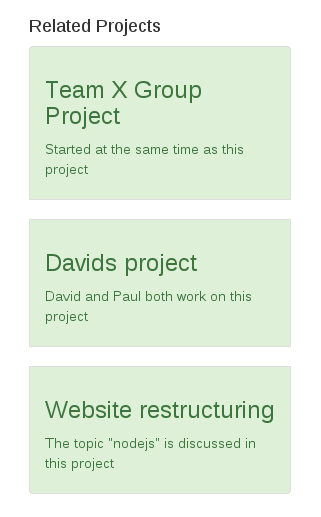
\includegraphics[scale = 0.8]{RelatedProj.png}
\centering
\caption{Example 'related projects' feature}
\label{fig:5}
\end{figure}

\section{Dashboards}

The various graphs and user metrics were grouped depending on their content.  The ones with information relating to the user's activity were added to a dashboard on the user profile (\ref{fig:12}).  The idea behind the dashboards was to provide a centralised hub for users to see their personal information, statistics about their contributions and suggested projects.  The page looks to group data logically, with one column devoted to graphs relating to the users activity, and another for information about the user and what they work on.

\begin{figure}[h]
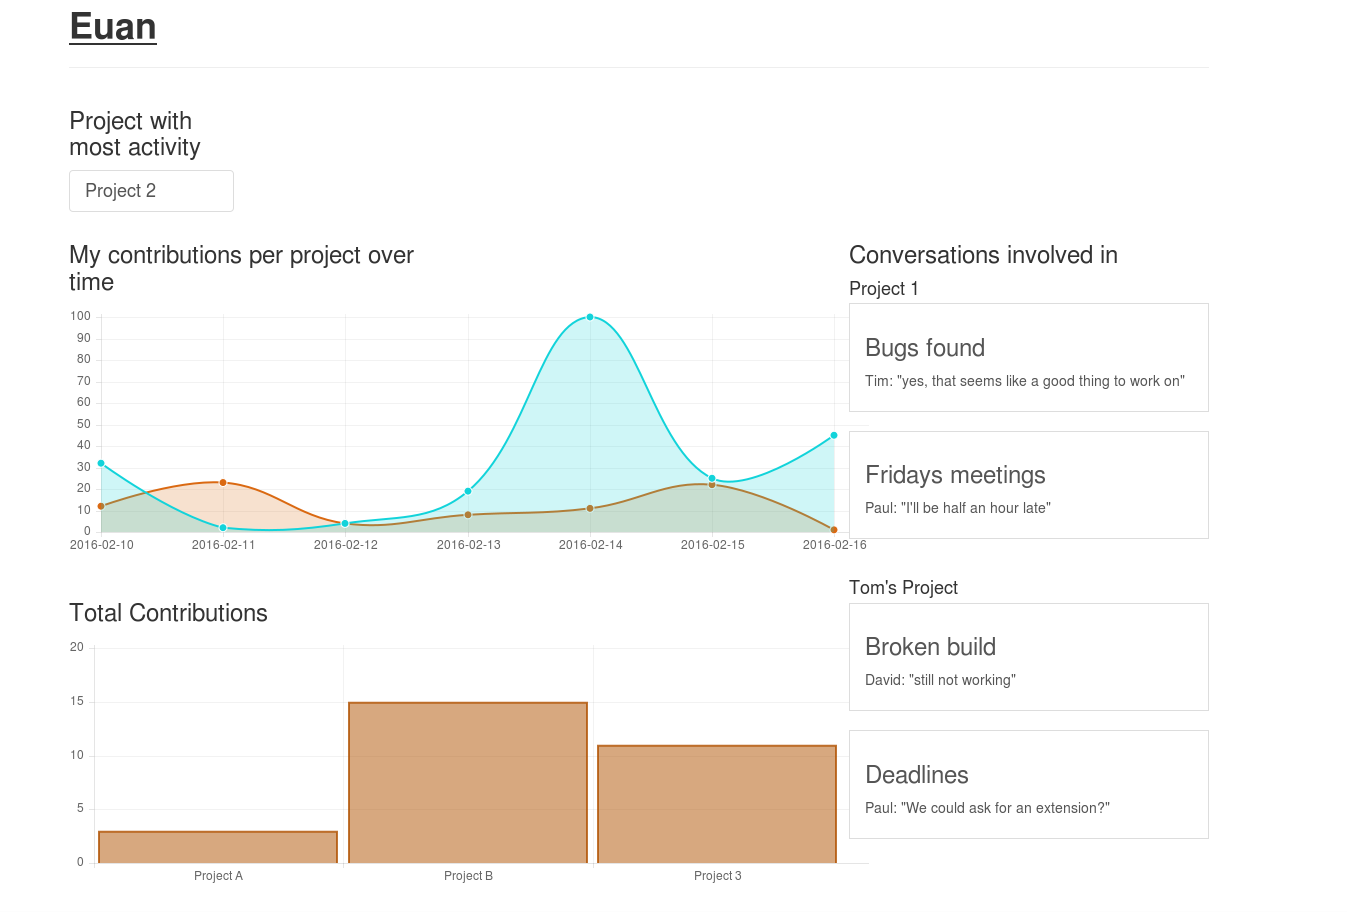
\includegraphics[scale=0.50]{profile-dashboard.png}
\centering
\caption{User dashboard partially populated with sample data}
\label{fig:12}
\end{figure}

\newpage

Similarly the project dashboard was built to gather all useful information about the project in one place (\ref{fig:11}).  A similar format to the user profile page is adopted, with the left-hand column being used to show a list of graphs relating to the project.  The first three graphs are fully implemented, and the remaining three are filled with sample data.  The right hand column shows related projects, suggested users and information about the project.

\begin{figure}[h]
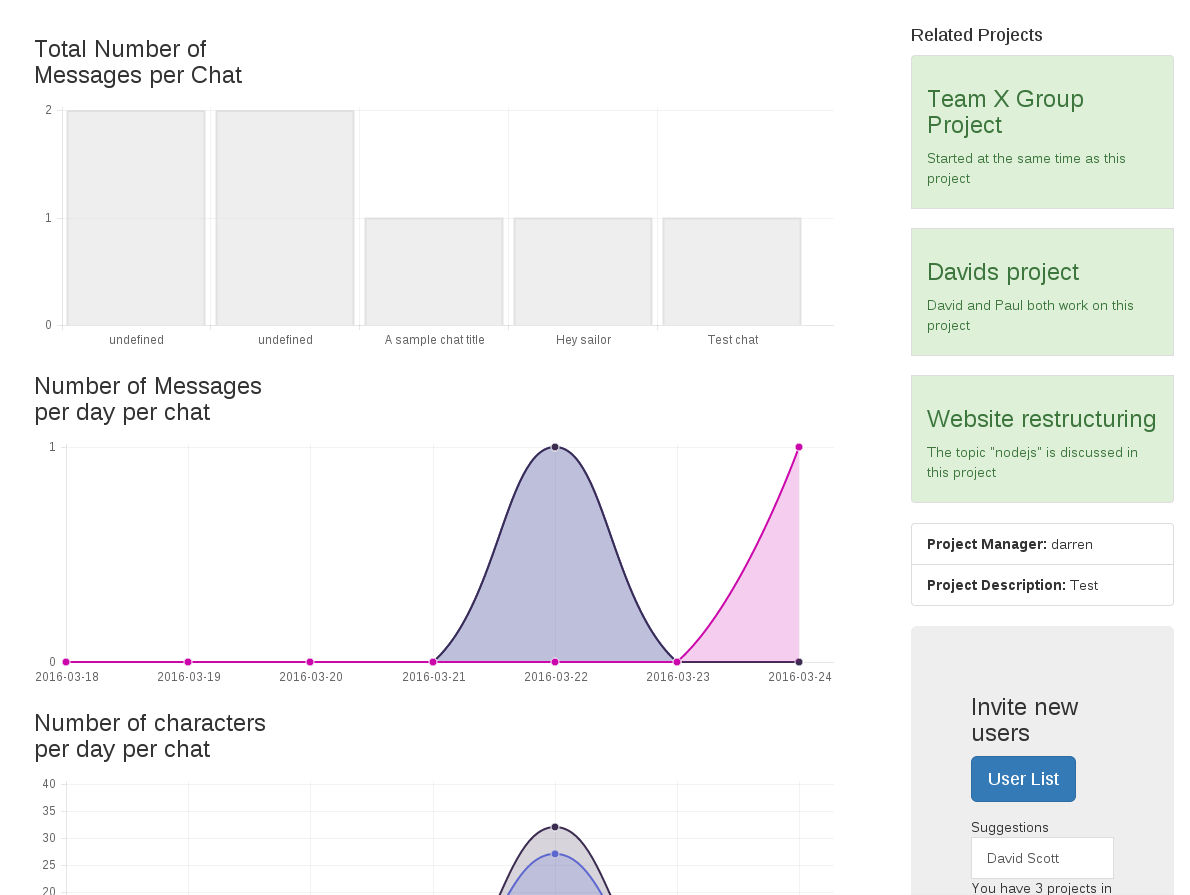
\includegraphics[scale=0.50]{project-dashboard.png}
\centering
\caption{Project dashboard populated with sample data}
\label{fig:11}
\end{figure}

\chapter{Future work}

The project could stand to benefit from a great deal of future work.  At present, a great number of the graphs and various suggestions are populated with sample data and as such these should be implemented properly for an actual release of the system.  The data analytics side of the system is yet to be fully explored, with only basic concepts being demoed in the current build. Moreover there is space for increasing the amount of graphs relating to the system, and the chat system could do with being further streamlined for easier communication.

\section{Analytics}

There could be an analysis of what a user frequently discusses, in order to build a profile of what sort of developer they are.  This information can be used to accurately recommend what sort of projects and conversations they should participate in, as well as recommend them to other users who are working in these areas.  Users that frequently work together or work on similar subjects could be recorded, and a tag could be added to the user profile denoting this, e.g. tags such as 'bug fixer', 'adds features' or 'documenter'. Similarly analysis of what is discussed in a project could be carried out.  This could be done by determining certain keywords that are frequently mentioned in conversations.  This information could be automatically added to the meta-data as a tag, or used in recommending related projects.

The information gathered in the graphs, such as the graph of 'Graph of content over time per chat' (\ref{fig:3}), could be used to categorise conversations.  For example, users could sort graphs according to which ones were worked on the most, or sort them by how recently they had been worked on.
Similarly the graphs such as 'graph of content over time per participant'(\ref{fig:4}) or 'total contributions' could be used to determine which members of a conversation participate the most in discussion, and as such this information would be useful in recommending users to add to other projects.

\newpage

\section {Graphs}
There are currently limitations in the graphing library used, namely in terms of customisation and variety in graphs, and in order to add new and more complex visualisations a different library should be adopted.  The current library only allows for six different chart types - bar, line, radar, polar area, pie and doughnut charts.  Although sufficient for the most usage, a greater variety in chart types could allow for different representations of data.


A network graph could be used to visualise how different users interact (\ref{fig:6}).  Each user would be represented as a node on the graph.  The user would be linked to other users that have a conversation in common with, and an overview of the graph could be used to view groups of users, as well as what sort of users work on what.  The colour of the connection could also denote the type of conversation they are linked by, e.g. a blue link for documentation, a yellow one for a feature, etc.
A bubble chart could be used to express conversations.  The size of each bubble could indicate the number of messages in the conversation, while the colour could show what type tag the conversation has.  This could be used to determine at a glance what sort of conversation a project predominantly consists of, as well as what sort of tag tends to have more discussion associated with it.



\begin{figure}[h]
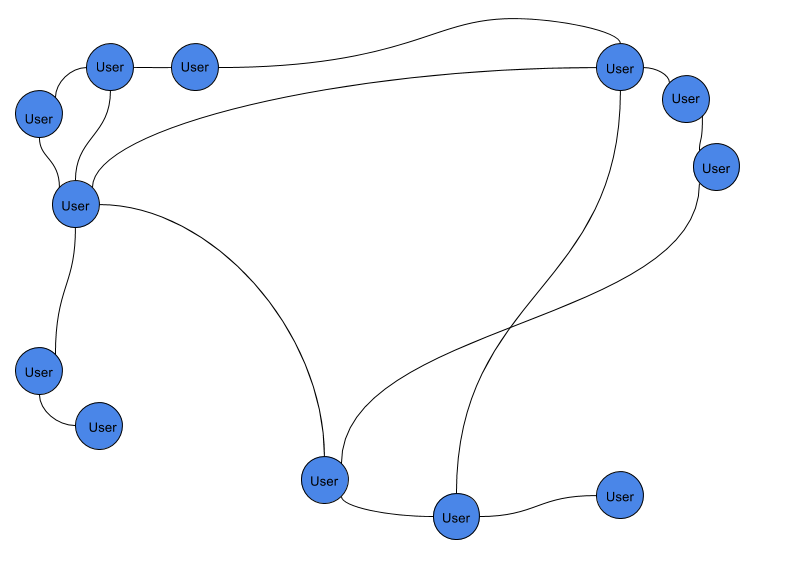
\includegraphics[scale = 0.5]{Proposed-graph.png}
\centering
\caption{Concept of future work for network graph}
\label{fig:6}
\end{figure}

\newpage

\section{Chat Features}

The chat system, although functionally complete, can be difficult to learn to use.  Despite the 'cheat sheet' (\ref{fig:13}) it can still be a challenge to remember the specific commands and as a result users may have to constantly refer back to the command list, which is a major inconvenience and one that takes up a lot of time.  Moreover, the project currently faces scalability problems whereby in a project with many participants it will be difficult for the user to remember multiple usernames in order to reference them in the chat.  

In response to this a useful feature to add would an auto-fill functionality.  This would assist new users in learning to use the system as it would show a list of all possible options when using features such as " \textasciicircum priority " and " \%tag ".  Moreover it would help fix the issues with large development teams, as users would not have to memorise each others usernames in order to tag them in the middle of discussions.  These 'quality of life' improvements are important for a system such as Tearooms, which aims to provide a service that emulates casual discussion as closely as possible, and as such ease of use and being simple to learn are imperative. 

\begin{figure}[h]
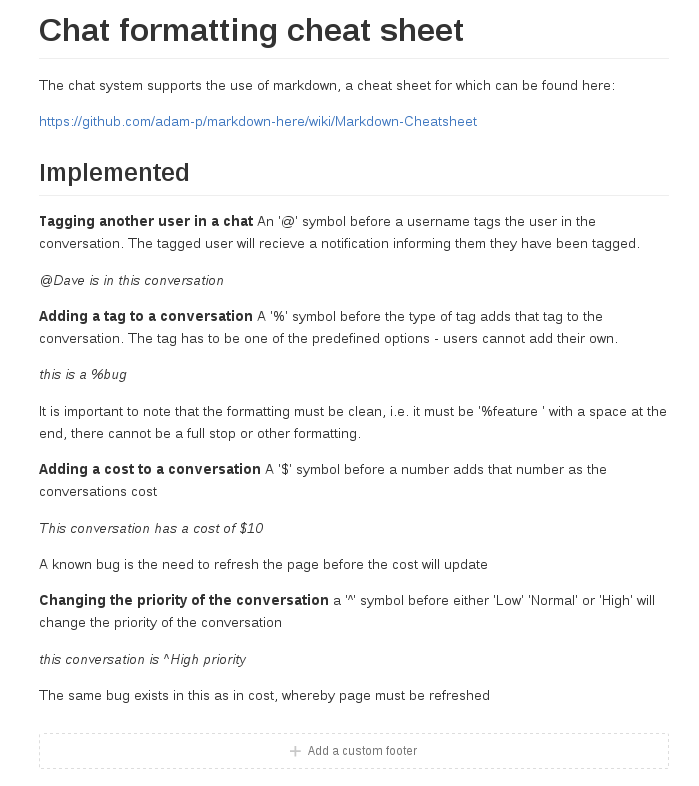
\includegraphics[scale = 0.7]{cheat-sheet.png}
\centering
\caption{Cheat sheet for the chat commands}
\label{fig:13}
\end{figure}

\newpage

\section{Analytics Quality Research}

The data analytics demoed in the project came about as a result of brief discussions with the project supervisor, and do not represent a comprehensive suite of useful features.  If this was to be developed further it would be necessary to carry out proper research on which analytics unearth the most useful information.  This could be done by looking at existing systems which offer similar features, such as Github (\ref{fig:14}). 


\begin{figure}[h]
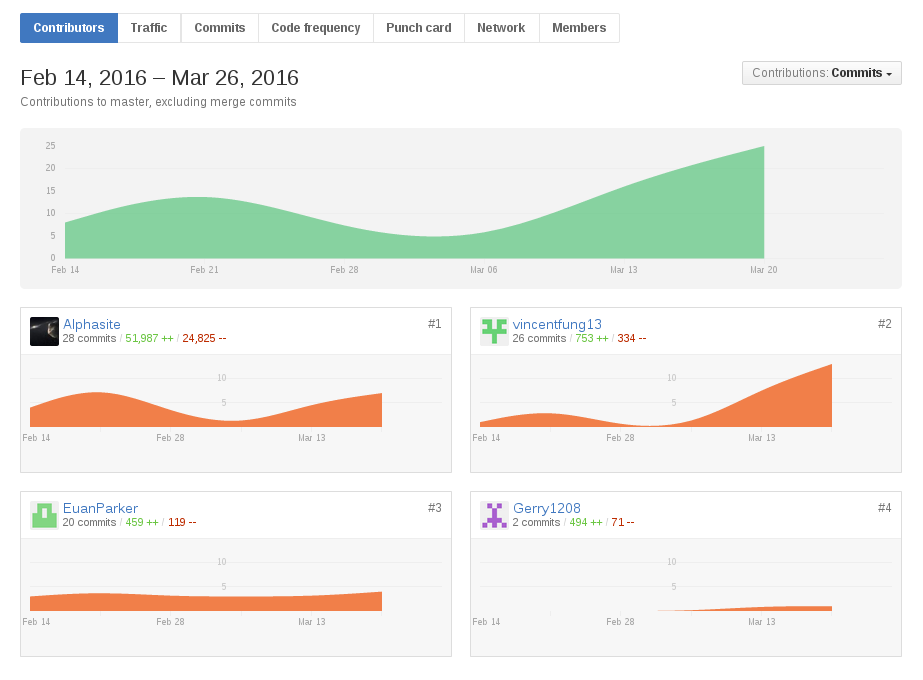
\includegraphics[scale = 0.7]{github-example.png}
\centering
\caption{Github graphs page}
\label{fig:14}
\end{figure}

Alternatively a number of the existing features (when properly implemented) could be trialled with an actual development team.  After having used the system for a period of time the team could be questioned on which ones they found the most useful.  
\chapter{Conclusion}

%%%%%%%%%%%%%%%% 
%              %
%  APPENDICES  %
%              %
%%%%%%%%%%%%%%%%
\begin{appendices}


\end{appendices}

%%%%%%%%%%%%%%%%%%%%
%   BIBLIOGRAPHY   %
%%%%%%%%%%%%%%%%%%%%

\bibliographystyle{plainnat}
\bibliography{l4proj}

\end{document}


